\section{Retrospective Findings}\label{sec:eval}
\noindent\textbf{Study setting.} We analyse \NExplanations{} saved explanations of \NFunctions{} functions: \NFuncApy{} from six Python repositories, \NFuncAjava{} from two Java repositories, and \NFuncB{} from EvalPlus, a benchmark of Python programming tasks~\cite{liu2023evalplus}. Repository functions span 5 to 45 lines at fixed revisions. We removed benchmark docstrings. We ran Qwen2.5-Coder-14B~\cite{hui2024qwencoder} and Qwen2.5-14B locally on all functions. Claude Haiku 5.5 covers three of five rounds. Fig.~\ref{fig:outcomes} abbreviates these explainers as Coder, Qwen and Haiku. Together they yield \NClaims{} extracted claims, including \RevLocalClaims{} from the two local models.

Qwen2.5-Coder extracts claims and generates probes from these explanations. Gemma2-9B and Llama3.1-8B separate Purpose from Rationale, agreeing on \RtAgree\% of cases (Cohen's chance-corrected agreement $\kappa=\RtKappa$). This measures model agreement. All rounds informed our checker development, making the results retrospective. Audits and corrected targets remain tentative assistant judgments pending independent human labels.

\subsection{Evidence coverage is concentrated in syntax and flow}
Our checker returns slot support or candidate refutation for \HoneFull\% [\HoneFullLo, \HoneFullHi] of local claims, including \HoneHeld\% [\HoneHeldLo, \HoneHeldHi] in the later three rounds. For these 95\% intervals, we resample whole functions 2,000 times, retaining their claims together. The intervals quantify function-resampling variability, excluding tuning uncertainty. Almost all of these outcomes indicate slot support (\DecTrueShare\%), but their reach varies by claim kind: outcome shares are \TypStructuralDec\% for structural claims and \TypDataflowDec\% for data flow, compared with below 1\% for behaviour.

Fig.~\ref{fig:outcomes} shows both this variation and claim composition: each bar represents one kind for one explainer, divided by outcome colour. Segment widths use the explainer's \emph{total} claims as denominator: the dark teal segment for Coder's structural claims, for instance, says that 24.6\% of all Coder claims are structural and slot-supported. The bar therefore shows this category's contribution to the full claim set. The large grey behavioural segments show where substantial content remains unchecked. Since rationale accounts for only \ResidRationale\% of local claims receiving neither outcome, our pipeline's missing support extends beyond design intent.
\begin{figure}[t]
\centering
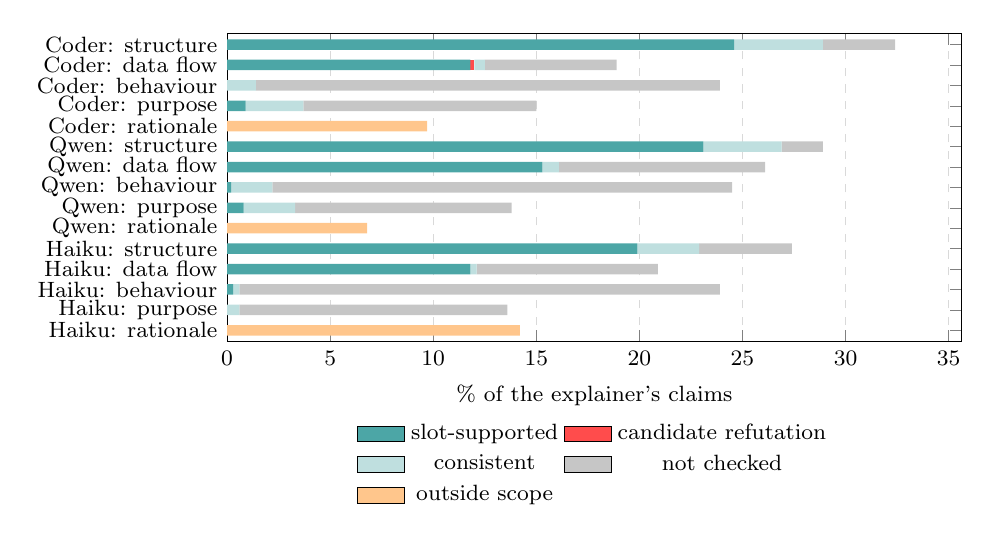
\begin{tikzpicture}
\begin{axis}[xbar stacked, width=0.90\columnwidth, height=5.5cm, bar width=3.8pt, xmin=0, xlabel={\% of the explainer's claims}, symbolic y coords={Haiku: rationale,Haiku: purpose,Haiku: behaviour,Haiku: data flow,Haiku: structure,Qwen: rationale,Qwen: purpose,Qwen: behaviour,Qwen: data flow,Qwen: structure,Coder: rationale,Coder: purpose,Coder: behaviour,Coder: data flow,Coder: structure}, ytick=data, yticklabel style={font=\footnotesize}, xticklabel style={font=\footnotesize}, label style={font=\footnotesize}, legend style={font=\footnotesize, at={(0.5,-0.23)}, anchor=north, legend columns=2, draw=none}, xmajorgrids, grid style={dashed,gray!30}, enlarge y limits=0.04]
\addplot[xbar,draw=none,fill=teal!70,area legend] coordinates {(24.6,Coder: structure) (11.8,Coder: data flow) (0.0,Coder: behaviour) (0.9,Coder: purpose) (0.0,Coder: rationale) (23.1,Qwen: structure) (15.3,Qwen: data flow) (0.2,Qwen: behaviour) (0.8,Qwen: purpose) (0.0,Qwen: rationale) (19.9,Haiku: structure) (11.8,Haiku: data flow) (0.3,Haiku: behaviour) (0.0,Haiku: purpose) (0.0,Haiku: rationale)};\addlegendentry{slot-supported}
\addplot[xbar,draw=none,fill=red!70,area legend] coordinates {(0.0,Coder: structure) (0.2,Coder: data flow) (0.0,Coder: behaviour) (0.0,Coder: purpose) (0.0,Coder: rationale) (0.0,Qwen: structure) (0.0,Qwen: data flow) (0.0,Qwen: behaviour) (0.0,Qwen: purpose) (0.0,Qwen: rationale) (0.0,Haiku: structure) (0.0,Haiku: data flow) (0.0,Haiku: behaviour) (0.0,Haiku: purpose) (0.0,Haiku: rationale)};\addlegendentry{candidate refutation}
\addplot[xbar,draw=none,fill=teal!25,area legend] coordinates {(4.3,Coder: structure) (0.5,Coder: data flow) (1.4,Coder: behaviour) (2.8,Coder: purpose) (0.0,Coder: rationale) (3.8,Qwen: structure) (0.8,Qwen: data flow) (2.0,Qwen: behaviour) (2.5,Qwen: purpose) (0.0,Qwen: rationale) (3.0,Haiku: structure) (0.3,Haiku: data flow) (0.3,Haiku: behaviour) (0.6,Haiku: purpose) (0.0,Haiku: rationale)};\addlegendentry{consistent}
\addplot[xbar,draw=none,fill=gray!45,area legend] coordinates {(3.5,Coder: structure) (6.4,Coder: data flow) (22.5,Coder: behaviour) (11.3,Coder: purpose) (0.0,Coder: rationale) (2.0,Qwen: structure) (10.0,Qwen: data flow) (22.3,Qwen: behaviour) (10.5,Qwen: purpose) (0.0,Qwen: rationale) (4.5,Haiku: structure) (8.8,Haiku: data flow) (23.3,Haiku: behaviour) (13.0,Haiku: purpose) (0.0,Haiku: rationale)};\addlegendentry{not checked}
\addplot[xbar,draw=none,fill=orange!45,area legend] coordinates {(0.0,Coder: structure) (0.0,Coder: data flow) (0.0,Coder: behaviour) (0.0,Coder: purpose) (9.7,Coder: rationale) (0.0,Qwen: structure) (0.0,Qwen: data flow) (0.0,Qwen: behaviour) (0.0,Qwen: purpose) (6.8,Qwen: rationale) (0.0,Haiku: structure) (0.0,Haiku: data flow) (0.0,Haiku: behaviour) (0.0,Haiku: purpose) (14.2,Haiku: rationale)};\addlegendentry{outside scope}
\end{axis}
\end{tikzpicture}
\caption{Claim composition and outcomes. Coder = Qwen2.5-Coder-14B, Qwen = Qwen2.5-14B and Haiku = Claude Haiku 5.5. Segment widths show each category's share of the explainer's total claims.}
\label{fig:outcomes}
\end{figure}


\subsection{Supported slots often leave sentence content unassessed}
We assess sentence-level alignment using a reproducible, seeded random sample of 40 of the \RevSupported{} local slot-supported verdicts. The assistant classified six as \emph{full-scope}, meaning that the evidence covered the sentence's assertions, 33 as asserting more than their slots and one as unrelated. Multiplying the supported share by the audited full-scope fraction gives our estimate across all local claims: $(\RevSupported/\RevLocalClaims)(6/40)=\RevFullShare\%$. Inverting the hypergeometric distribution for sampling without replacement gives a 95\% finite-population interval [\RevFullLo, \RevFullHi]. This interval conditions on our corpus and tentative labels. Sentence truth still requires a separate assessment.

\begin{table}[t]\centering\caption{Policy coverage among all 822 local claims. Audit mismatch counts partial/unrelated judgments over audited accepted claims. Sentence truth requires separate assessment.}\label{tab:risk}\footnotesize\begin{tabular}{@{}lrr@{}}\toprule Policy & Coverage \% & Audit mismatch \\\midrule
Exact syntax baseline & 18.9 & 20/20 \\
Exact structural support & 23.5 & 23/27 \\
Structural + flow support & 37.3 & 34/39 \\
All supported outcomes & 38.3 & 34/40 \\\bottomrule\end{tabular}\end{table}

These mismatches led us to compare four fixed display \emph{policies}, each selecting which results to show (Table~\ref{tab:risk}). Our syntax baseline directly matches extracted call or parameter names, whereas the other policies accept supported outcomes from exact structural rules, structural plus data-flow rules, or all rules. Coverage divides accepted claims by all \RevLocalClaims{} local claims. ``Audit mismatch'' divides partial/unrelated judgments by audited accepted claims. Thus displaying all supported outcomes covers 38.3\%, with 34 mismatches among 40 audited cases. The baseline accepts less, yet all 20 of its audited cases mismatch. These counts describe scope mismatch. Sentence truth and slot correctness require separate validation. Our bounds allow unaudited labels to take either value.

\subsection{Extracted representations change checker outcomes}
\begin{table}[t]
\centering\caption{Planted pairs: original and altered statements. Unmatched counts failed extractions over both twins. Candidate refutation and slot support count altered twins only. Construction (nominal) truth labels are unvalidated.}
\label{tab:planted}\footnotesize\setlength{\tabcolsep}{3pt}
\begin{tabular}{@{}lrrrr@{}}\toprule
Pair set & Pairs & Unmatched & \shortstack{Candidate\\refutation} & \shortstack{Slot\\support} \\\midrule
All frozen (nominal) & 151 & 26/302 & 44/151 & 33/151 \\
No known label errors & 148 & 26/296 & 43/148 & 31/148 \\
Original supported & 116 & 24/232 & 42/116 & 28/116 \\
\bottomrule\end{tabular}\end{table}

To investigate where mismatches begin, we use \emph{planted pairs}: an original statement and a deliberately altered counterpart, whose members we call \emph{twins}. Their \emph{nominal} true/false labels inherit construction and engine judgments and await independent validation. We retain all 151 pairs in Table~\ref{tab:planted}. Removing three assistant-identified label-error pairs gives its second row. Further excluding 32 pairs whose originals no longer receive slot support leaves the 116 pairs in its last row. Targeted assistant audits cover 31 pairs.

In the complete set, extraction failed to match 26 of 302 twins, while 44 of 151 altered twins received candidate refutation and 33 received slot support. The different denominators matter: ``Unmatched'' counts both twins, but refutation and support count altered twins only. These pair sets expose selection effects without resolving nominal-label uncertainty.

Holding the checker and facts fixed, we next change only the extracted targets. An assistant prepared and froze corrected targets for all \RevAblPairs{} structural/data-flow pairs (\RevAblTwins{} twins), retaining sentences, conditions and receivers, the objects on which methods are called. The annotations mark \RevAblUnrep{} twins as unrepresentable by one faithful target. These corrections start from the original slots, so they are neither blinded nor independently validated reference (``gold'') annotations.

With those corrected targets, Slot-supported outcomes on nominal altered twins fall from \RevAblBefore{} to \RevAblAfter{}. The original extraction leaves \RevAblLost{} twins unmatched. These transitions measure representation sensitivity. Residual support may concern another subclaim or reflect a wrong label or checker error. In the five remaining cases, assistant inspection found confused name/role matches, unchecked conditions and confusion between converting a value and passing it along. We retain each twin's before/after outcomes and examples in the artifact.

How often false claims occur also matters. Refutation \emph{precision}, the fraction of candidate refutations assigned a nominal false label, is \RevPrecHalf\% in our selected-pair sensitivity calculation when 50\% of claims are assumed false. It falls to \RevPrecOne\%, \RevPrecFive\% and \RevPrecTen\% at 1\%, 5\% and 10\%, respectively: when false claims are rare, contradictions issued on true claims can dominate the alerts. These calculations describe assumed prevalence scenarios. Deployment estimates would require representative data. Our current corpus contains one candidate refutation, judged correct by the assistant after rules were revised using this corpus. Our artifact includes function-resampling intervals and the 25\% scenario.
